\fancyhead[R]{\textsc{Key Comments}}
\rfoot{\textsc{Page \thepage}}

\par
Prior to this article, Lawrence Summers arguably had astounding educational backround, 
as well as attending Massachusetts Institute of Technonogy (MIT) at an early age of 16.
Shortly after MIT, he attended Harvard University as a graduate earning his (Ph.D., 1982),
but also become one of youngest professor at age of 28.\cite{summersedu} As for his
professional career, working closely with Clintion's administration as Treasury 
Secretary~\cite{ustreasury} and Obama administration as director of the National Economic
Concil,\cite{economicconcil} well accomplished would be an understatement.

\par
Fastward to the cause of article written by PBS NewsHour, \say{Harvard President Summers’ 
Remarks About Women in Science, Engineering},\cite{summers} appears that the Harvard 
President at that time, Lawrence Summers gotten himself into a controversial predicament 
even after 15 years talked about today. A problem that caught the interest of Summers, 
lead to him addressing why wonmen are underrepresented particularly in the science and 
engineering. In doing so, he wanted to, \say{\dots, attempt to adopt an entirely positive, 
rather than normative approach, \dots,\cite{summers}} provoke his audience. In attempt to
analyze and breakdown three hypotheses listed in order of importance rank, according to 
Summers~\cite{summers}: 
\say{
  (1) \emph{high-powered job hypothesis}, 
  (2) \emph{availability of aptitude hypothesis}, and 
  (3) \emph{socialization and patterns of discrimination hypothesis}}.

\par
His most important hypothesis, also known as the \say{(1) high-powered job hypothesis},
claims that: \say{\dots there are many professions and many activities, and the most 
prestigious activities in our society expect of people who are going to rise to leadership 
positions in their 40s near total commitments to their work.}\cite{summers}. Then later,
he questions our society for desires of prominent jobs. The pattern he observes is apparently
men who desire \say{high-powered intense work}\cite{summers}. To summerize what I think he
meant is, women do not desire for high-powered work since they prefer to get married and 
prioritize rasining a family. A young women who had worked closely with him at the Treasury,
reported from her graduate class at Harvard, only 3 out of 22 women are working full time 
currently. From this small sample size, he is certain that \say{(1) high-powered job hypotheis}
flavor torwards men.

\par
Without a doubt, \say{(2) availability of aptitude hypotheis} is the reason for most negative 
criticism and controversial debate on matter of lack thereof women in stem fields. While watching
Professor Susan Williams, she paraphrased Summers statements on aptitude, \say{\dots innately thus 
genetically different from men and lacked natural ability of men in these fields\dots}\cite{williams}.
Her expression in disbelief that someone in his caliber could say such ridicule comment, went into
history of why women are underrepresented. She then compares Summers with Aristotle, after all these
years women still burden this stigma that men are more superior. Nonetheless, Summers and many men
alike, often reference such claim by \say{greater male variability hypothesis}. As stated by Summers,
\say{If you do that calculation — and I have no reason to think that it couldn’t be refined in a 
hundred ways — you get five to one, at the high end.}\cite{summers} To visually understand this
concept, provided below are two distribution curves with exact same means. However, it differs in
variabilities, the green (\textcolor{darkpastelgreen}{males}) curve showing that males have both
the lowest and highest test results.

\begin{center}
  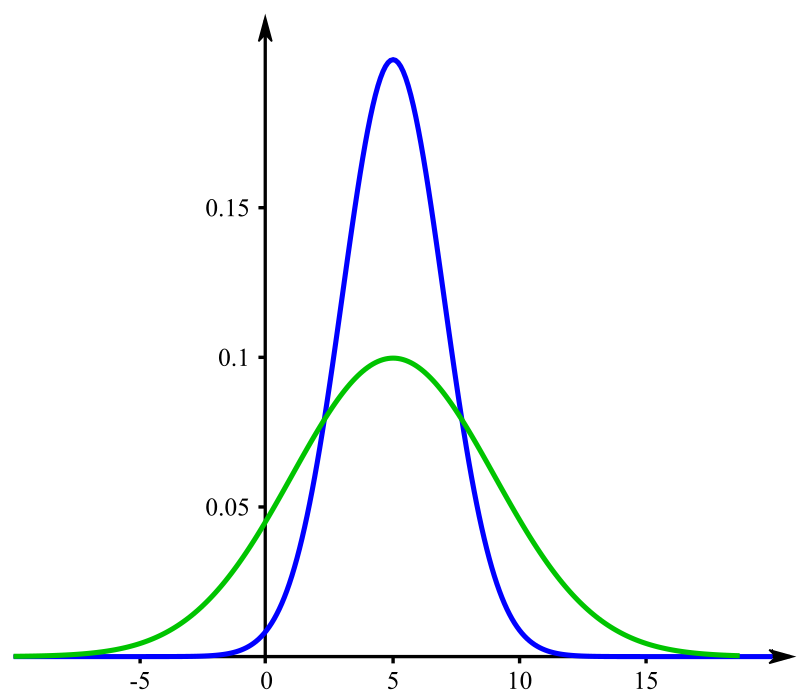
\includegraphics[width=0.2\textwidth]{normaldis.png}
\end{center}

\par
Lastly, socialization and patterns of discrimination, Summers described as girls are socialized
towards nursing while boys are towards building bridges. However, according to him, \say{there are 
issues of intrinsic aptitude, and particularly of the variability of aptitude, and that those 
considerations are reinforced by what are in fact lesser factors involving socialization and continuing 
discrimination.} He believes \say{(3) socialization and patterns of discrimination hypothesis} is
not part of the contribution, if any, towards undermining of women in stem fields.

\clearpage